\documentclass{article}
\usepackage[utf8]{inputenc}
\usepackage[margin=3cm]{geometry}
\usepackage{indentfirst}
\usepackage{graphicx}
\usepackage{amsmath}
\graphicspath{ {./images_a3/} }
\setlength{\parindent}{0.75cm} %heh, 0.75

\title{
    \textbf{Programação 3D - Assignment III}
    }
\author{
    \begin{Large}
        \textbf{Grupo 02}
    \end{Large}\\
    Francisco Campaniço 83463\\
    João Rafael 83482\\
    Rodrigo Oliveira 83558
}
\date{Maio 2019}

\begin{document}

    \maketitle
    \begin{figure}[h]\begin{center}
        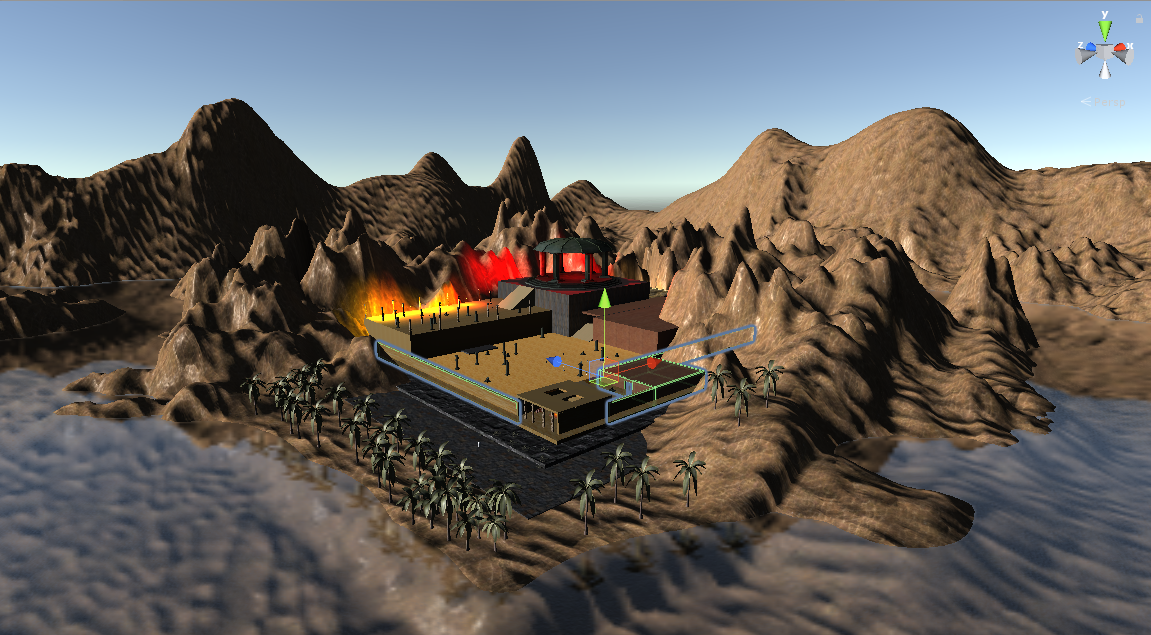
\includegraphics[scale=0.27]{Screenshot_1.png}
        \caption{A cena de jogo.}
    \end{center}\end{figure}

    \section*{\textit{Start / End Screens}}
        \par
        Ao abrir o jogo, aparece um ecrã de início simples com um botão "start". Este ecrã trata-se de uma cena separada do jogo principal, e quando o jogador carrega no botão, a cena muda para a principal.
        \par
        Ao acabar o jogo (quer por o jogador ficar com zero vida ou chegar ao fim do nível), aparece um ecrã de fim, indicando a pontuação do jogador num \textit{leaderboard}.
    \section*{HUD}
        \begin{figure}[h]\begin{center}
            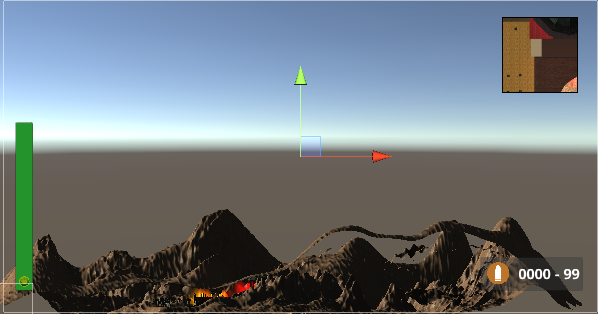
\includegraphics[scale=0.4]{Screenshot_3.png}
            \caption{HUD.}
        \end{center}\end{figure}
        \par
        O HUD mostra uma barra com a vida do jogador, um contador de munição da arma e um minimapa.
        \par
        O minimapa e feito com uma câmara ortográfica a ver a posição do jogador de cima. A câmara envia a informação para uma \textit{raw texture} situada no HUD.

    \section*{Colisões}
        \par
        O jogador pode disparar sobre barris explosivos para causar uma explosão. Se houverem vários barris perto uns dos outros, dá-se uma explosão em cadeia. As explosões também repelem outros \textit{rigidbodies} aos quais se aplicam físicas de jogo, e tiram metade da vida do jogador.
        \par
        O jogador pode pegar em objetos ao manter premida a roda do rato (\textit{MouseButton3}). Esta funcionalidade usa o \textit{raycasting} do Unity para verificar se o jogador está a apontar para um \textit{rigidbody}.
        \par
        Uma das salas do jogo está escura até o jogador passar por \textit{triggers} escondidos na sala, que ativam \textit{spotlights} (usando \texttt{OnTriggerEnter()}).
        \par
        Há um "elevador" que, quando o jogador se posiciona em cima do mesmo, eleva-se até o jogador sair ou até a um limite dado por um \textit{collider} invisível. (Usa-se \texttt{OnTriggerEnter()}, \texttt{OnTriggerStay()} e \texttt{OnTriggerExit()}.)
        \par
        Existem \textit{turrets} que disparam balas para o jogador. Estes seguem a posição do jogador, rodando na usa direção se ele se mexer.
        \begin{figure}[h]\begin{center}
            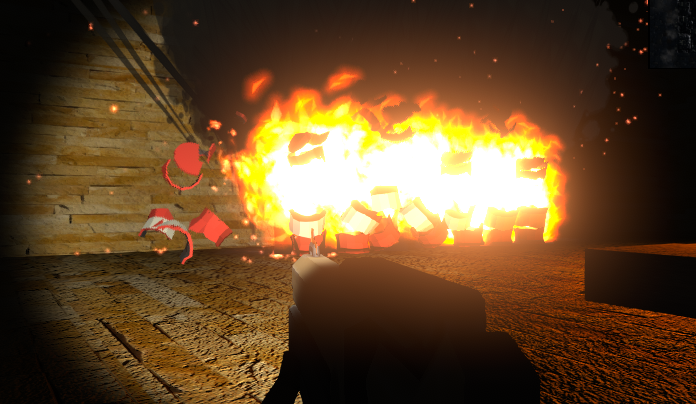
\includegraphics[scale=0.3]{Screenshot_4.png}
            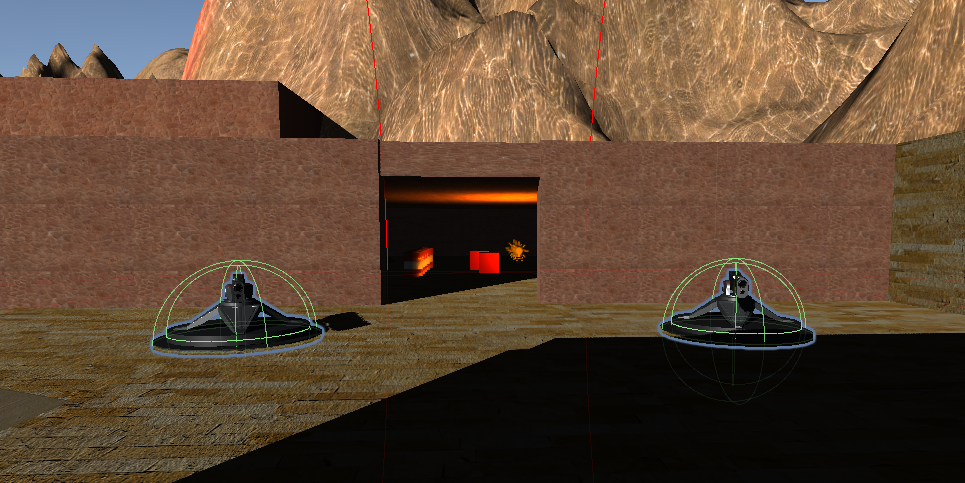
\includegraphics[scale=0.25]{Screenshot_5.png}
            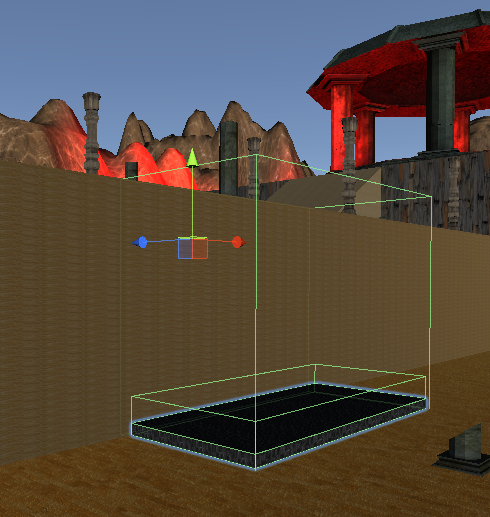
\includegraphics[scale=0.23]{Screenshot_6.png}
            \caption{Barris explosivos, \textit{turrets} e elevadores.}
        \end{center}\end{figure}
    \section*{Mecânicas de jogo}
        \par
        O jogador tem uma arma com munições finitas, e 100 pontos de vida. Caso os pontos de vida cheguem a zero, o jogador morre e chega-se ao ecrã de fim. Estar perto de uma explosão tira 50 pontos de vida, e levar com uma bala ou ser atacado por um esqueleto tira 10 pontos. Se o jogador interagir com uma caixa de munições, ganha 100 balas extra para a arma.
        \par
        Se chegar à "sala do tesouro", a pontuação do jogador duplica. A pontuação baseia-se no tempo desde o jogo começar.
    \section*{Efeitos Visuais}
        \par
        O  \textbf{\textit{bump mapping}} é feito por aplicar uma textura normal (\textit{normal map}) ao material de certos elementos de jogo.
        \par
        As \textbf{\textit{lens flares}} são aplicadas à \textit{directional light}, para parecer como um "sol".
        \par
        O \textbf{\textit{environment mapping}} é feito através de uma reflection probe, cujo \textit{environment map} é aplicado a uma esfera para demonstração.
        \begin{figure}[h]\begin{center}
            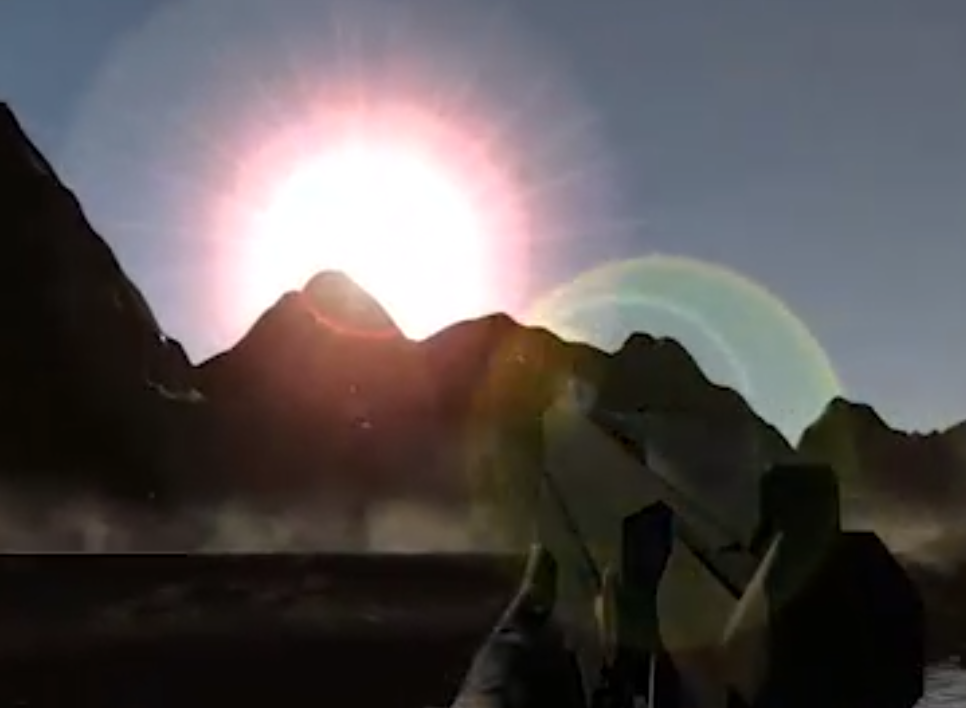
\includegraphics[scale=0.15]{flares.png}
            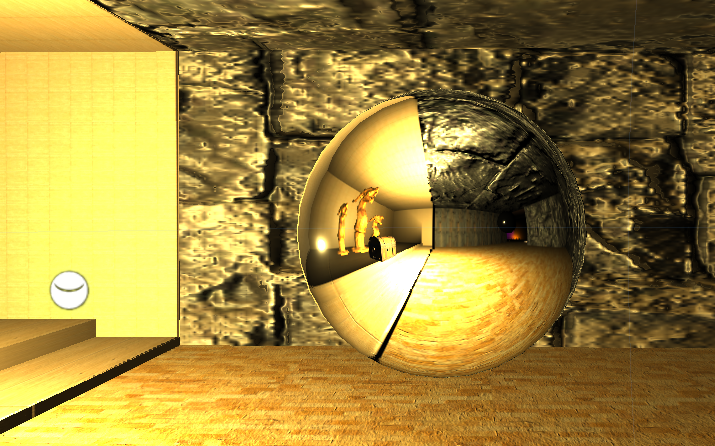
\includegraphics[scale=0.24]{Screenshot_2.png}
            \caption{\textit{Lens flares, environment mapping}.}
        \end{center}\end{figure}
        \par
        Usam-se vários sistemas de \textbf{partículas} do Unity, como vapor, fogo e explosões.
        \par
        O Unity tem uma \textit{stack} de pós-processamento incluída. Isto permite a adição de \textbf{\textit{ambient occlusion}} e \textbf{\textit{HDR bloom}} ao jogo. A \textit{bloom} tem um \textit{threshold} alto, e só é visível em luzes intensas (numa explosão, por exemplo). O componente HDR tem cor branca, aumentando a intensidade para branco quando há bloom no ecrã.
        \begin{figure}[h]\begin{center}
            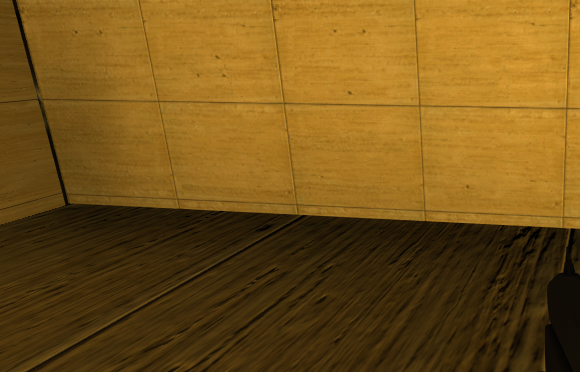
\includegraphics[scale=0.34]{Screenshot_21.png}
            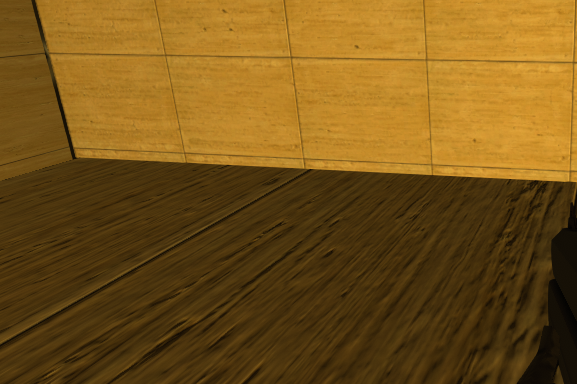
\includegraphics[scale=0.33]{Screenshot_22.png}
            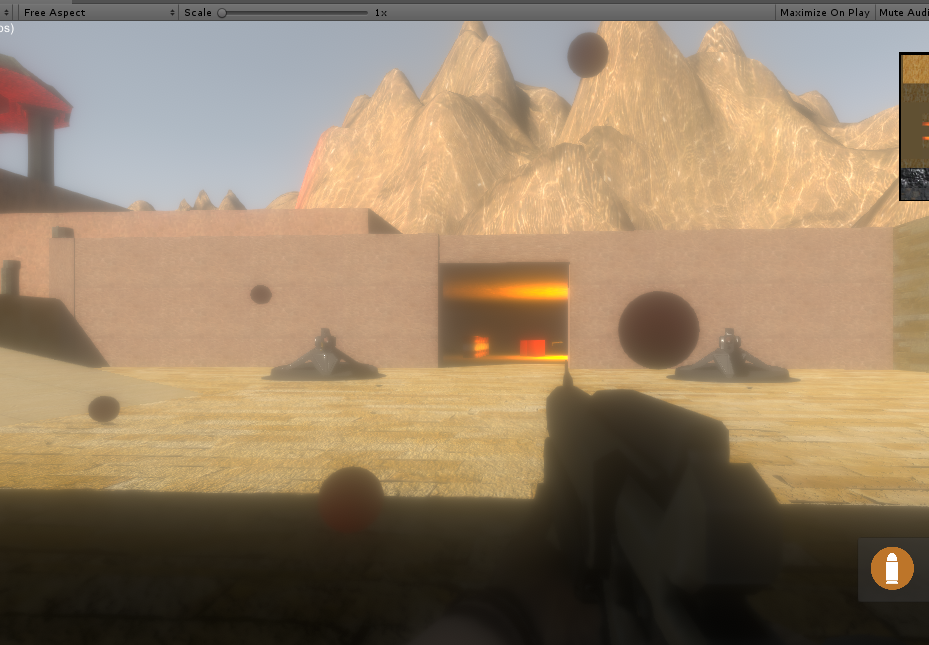
\includegraphics[scale=0.2]{Screenshot_18.png}
            \caption{\textit{Ambient Occlusion} ligado/desligado, \textit{bloom}.}
        \end{center}\end{figure}
        \subsection*{Iluminação Global}
        \par
        Para \textbf{\textit{realtime lighting/shadows}} aplica-se a grande parte das luzes a propriedade \textit{"realtime"}. Isto inclui, por exemplo, o "sol", o que dá origem a uma espécie de ciclo dia-noite, dado que a luz direcional que representa um sol roda á volta do nível, afetando a posição das sombras no nível todo.
        \par
        Para \textbf{\textit{baked lighting}}, aplicou-se a uma point light vermelha no topo do nível a propriedade "baked", assegurando que a geometria à sua volta têm um \textit{lightmap} aplicado que é computado no \textit{engine}, antes da execução do jogo.
        \begin{figure}[h]\begin{center}
            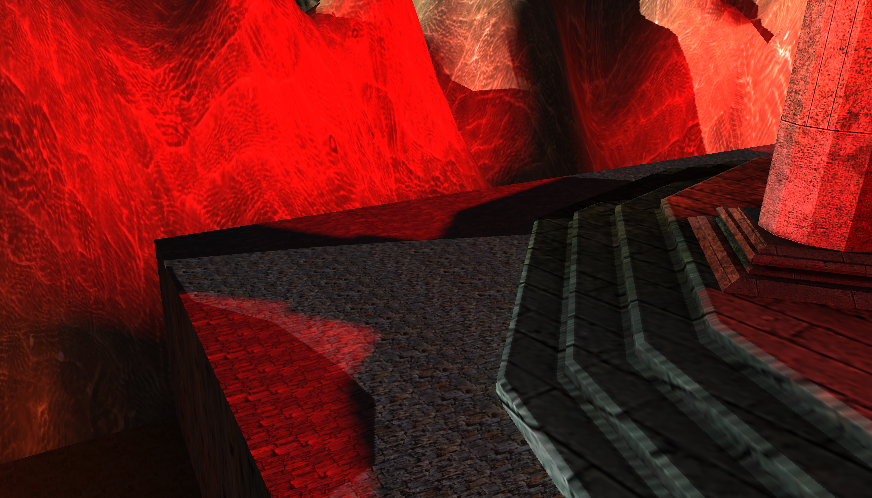
\includegraphics[scale=0.25]{Screenshot_9.png}
            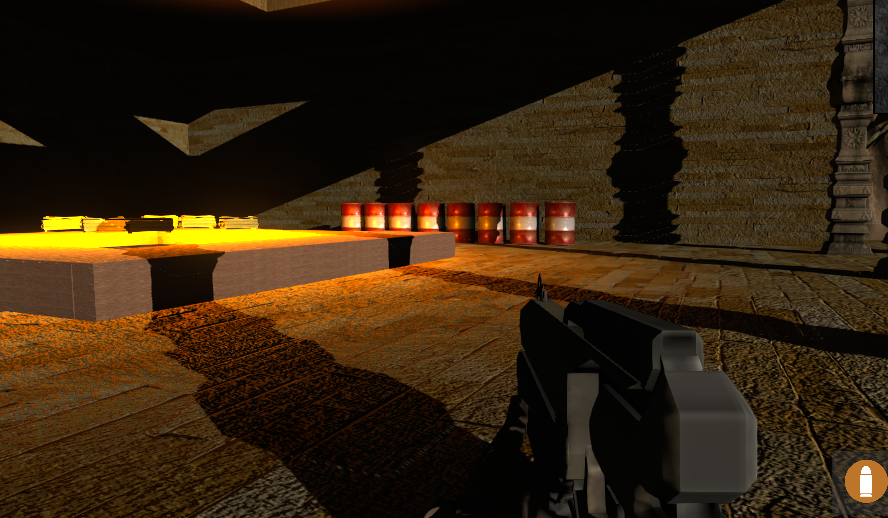
\includegraphics[scale=0.24]{Screenshot_14.png}
            \caption{\textit{Baked/realtime shadows}.}
        \end{center}\end{figure}

    \section*{Extras}
        \par
        Dado o componente de Pós-processamento do Unity, também adicionámos \textbf{\textit{motion blur}} e \textbf{\textit{color grading}} ao jogo, tal como \textbf{\textit{depth of field}}, que só se ativa quando o jogador carrega no botão direito do rato e olha pela mira da arma (simulando a falta de foco na arma em si). Também foi adicionado scripting à \textit{bloom}: se o jogador perder vida, o \textit{threshold} baixa e a intensidade aumenta temporariamente, como se a personagem tivesse sido "atordoada".
        \begin{figure}[h]\begin{center}
            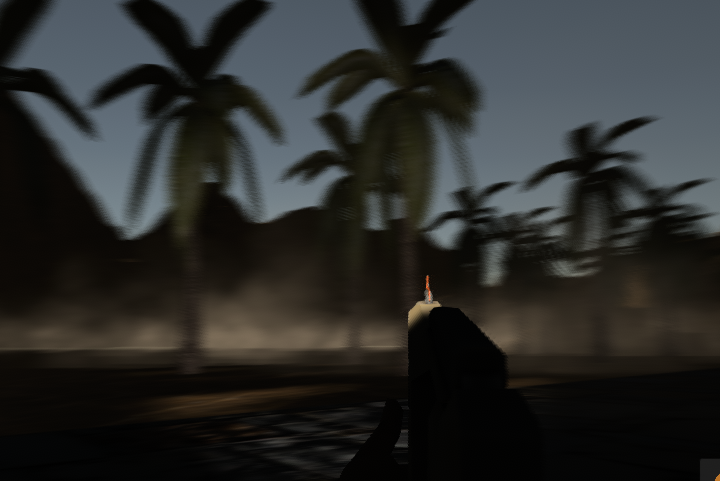
\includegraphics[scale=0.3]{Screenshot_13.png}
            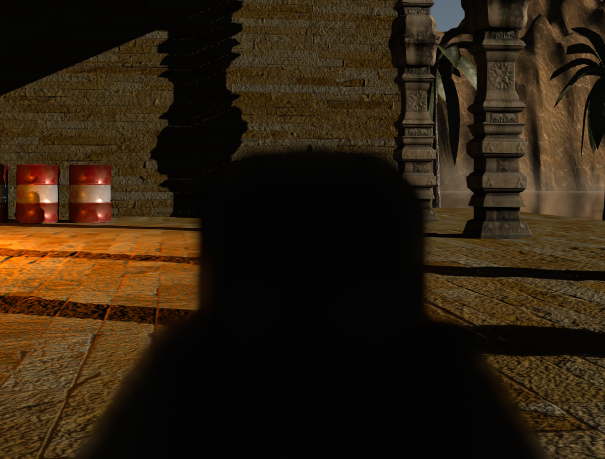
\includegraphics[scale=0.315]{Screenshot_15.png}
            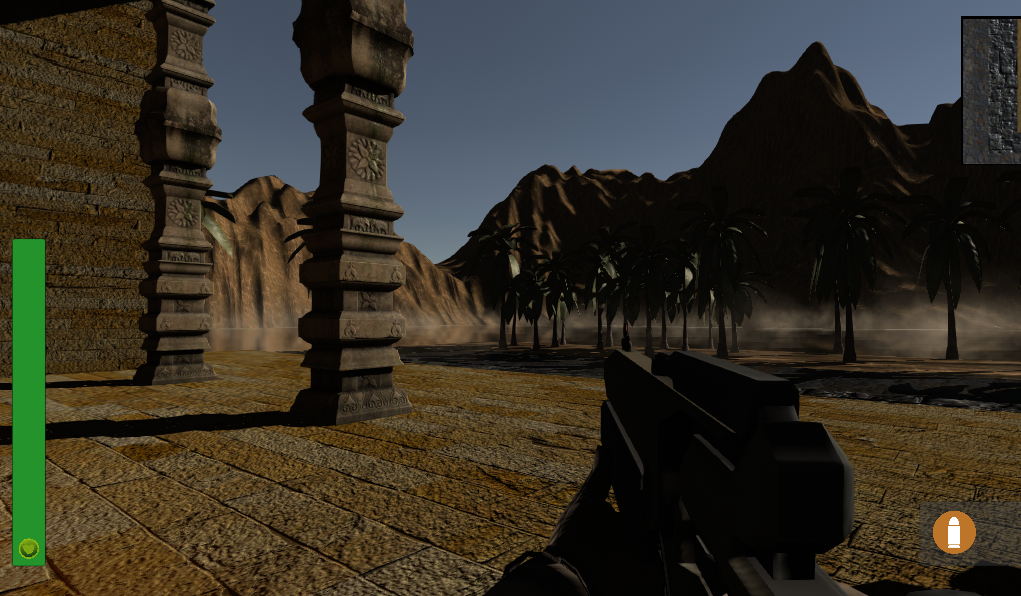
\includegraphics[scale=0.2]{Screenshot_16.png}
            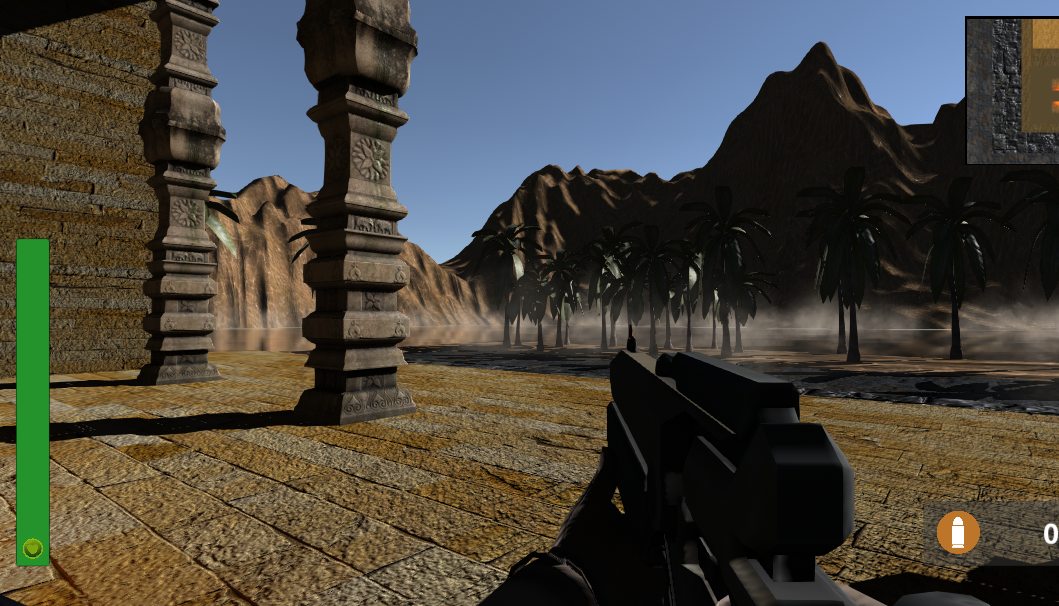
\includegraphics[scale=0.1955]{Screenshot_17.png}
            \caption{\textit{Motion blur, depth of field} e \textit{color grading} ligado/desligado.}
        \end{center}\end{figure}
        \par
        Além de \textit{turrets}, existem esqueletos que seguem o jogador e tentam atacá-lo. Estes esqueletos podem mexer-se por uma \textit{navmesh}, que é pré-computada, e consiste das \textit{meshes} que foram marcadas como "navigation static". Os esqueletos também tem as suas próprias barras de vida.
        \par
        A ilha onde se passa o jogo está rodeada de água, que tem \textit{screen-space reflections}.
        \par
        Há uma parte do nível com esferas que se mexem sozinhas, seguindo uma animação.
        \par
        Quando o jogador é atingido por uma bala, aparecem esferas vermelhas a simular "sangue".
        \begin{figure}[h]\begin{center}
            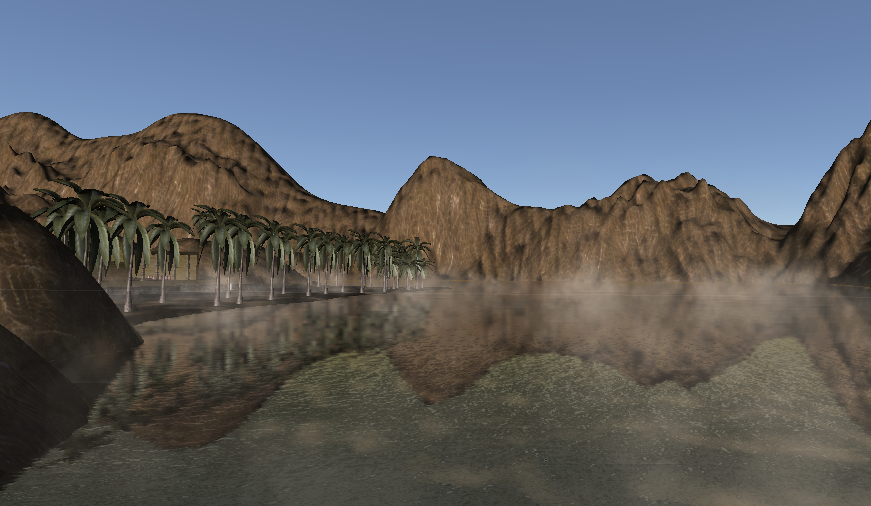
\includegraphics[scale=0.2]{Screenshot_12.png}
            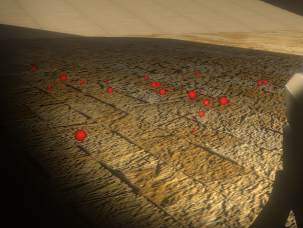
\includegraphics[scale=0.445]{Screenshot_19.png}
            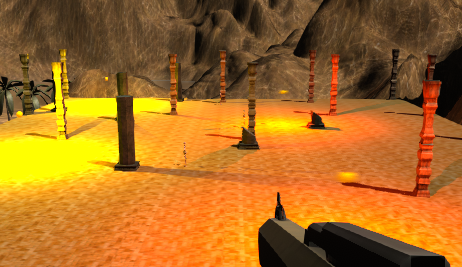
\includegraphics[scale=0.38]{Screenshot_23.png}
            \caption{\textit{Screen-space reflections}, esferas de "sangue" e esferas em movimento.}
        \end{center}\end{figure}


\end{document}